\documentclass[answers,12pt,addpoints]{exam}
\usepackage{import}

\import{C:/Users/prana/OneDrive/Desktop/MathNotes}{style.tex}

\newcommand{\RR}{\mathbb{R}}
\newcommand{\EE}{\mathbb{E}}
\newcommand{\TV}{\mathrm{TV}}

% Header
\newcommand{\name}{Pranav Tikkawar}
\newcommand{\course}{Stat 654}
\newcommand{\assignment}{Homework 5}
\author{\name}
\title{\course\ - \assignment}

\begin{document}
\maketitle

%%%%%%%%%%%%%%%%%%%%%%%%%%%%%%%%%%%%%%%%%%%%%%%%%%%%%%
\section*{Problem 1: Gaussian couplings}

Recall that a coupling of two random variables with given marginals means a joint construction of them on the same probability space. Let $X, Y \sim N(0,1)$ be two independent $N(0,1)$ random variables.

\begin{enumerate}
  \item Let $Z := aX + bY$. You may use without proof that $Z$ is also Gaussian. Compute the mean and variance of $Z$. For what condition on $a$ and $b$ does $Z$ have distribution $N(0,1)$?

  \begin{solution}
  Let $Z := aX + bY$ with $X,Y \sim N(0,1)$ independent. Then
  \[
  \EE[Z] = a\EE[X] + b\EE[Y] = 0.
  \]
  Also,
  \[
  \Var(Z) = a^2\Var(X) + b^2\Var(Y) + 2ab\Cov(X,Y).
  \]
  Since $X$ and $Y$ are independent, $\Cov(X,Y)=0$, and since $\Var(X)=\Var(Y)=1$, we get
  \[
  \Var(Z) = a^2 + b^2.
  \]
  Therefore $Z \sim N(0,1)$ if and only if
  \[
  a^2 + b^2 = 1.
  \]
  \end{solution}

  \item Show that $(X,\rho X + \sqrt{1-\rho^2}\,Y)$ is a coupling of two standard Gaussian random variables for any $\rho \in [-1,1]$. Draw a scatterplot of the pair and plot histograms of both coordinates to numerically verify that each marginal distribution is standard Gaussian. This coupling is called the identical coupling when $\rho = 1$, the independent coupling when $\rho = 0$, and the antithetic coupling when $\rho = -1$.

  \begin{solution}
Define
\[
  Z_\rho := \rho X + \sqrt{1-\rho^2}\,Y, \qquad \rho \in [-1,1].
\]
Then
\[
  \mathbb{E}[Z_\rho]
  = \rho \mathbb{E}[X] + \sqrt{1-\rho^2}\,\mathbb{E}[Y]
  = 0,
\]
and
\[
  \operatorname{Var}(Z_\rho)
  = \rho^2 \operatorname{Var}(X)
    + (1-\rho^2)\operatorname{Var}(Y)
    + 2\rho\sqrt{1-\rho^2}\,\operatorname{Cov}(X,Y)
  = \rho^2 + (1-\rho^2) = 1,
\]
since $X$ and $Y$ are independent with
$\operatorname{Var}(X)=\operatorname{Var}(Y)=1$ and
$\operatorname{Cov}(X,Y)=0$.
Hence $Z_\rho \sim N(0,1)$, so $(X,Z_\rho)$ is a coupling of two
standard Gaussian random variables for every $\rho \in [-1,1]$.

\medskip

For a numerical verification, we simulate $n = 10^5$ i.i.d.\ pairs
$(X_i,Y_i)$ from $N(0,1)$ and form
\[
  Z_{\rho,i} := \rho X_i + \sqrt{1-\rho^2}\,Y_i, \qquad i=1,\dots,n,
\]
for three values $\rho \in \{1,0,-1\}$.  The following R (or Python)
code generates scatterplots of $(X_i,Z_{\rho,i})$ and overlaid
histograms of the marginals $X$ and $Z_\rho$.

\medskip


The resulting figures are included below.

  \begin{center}
    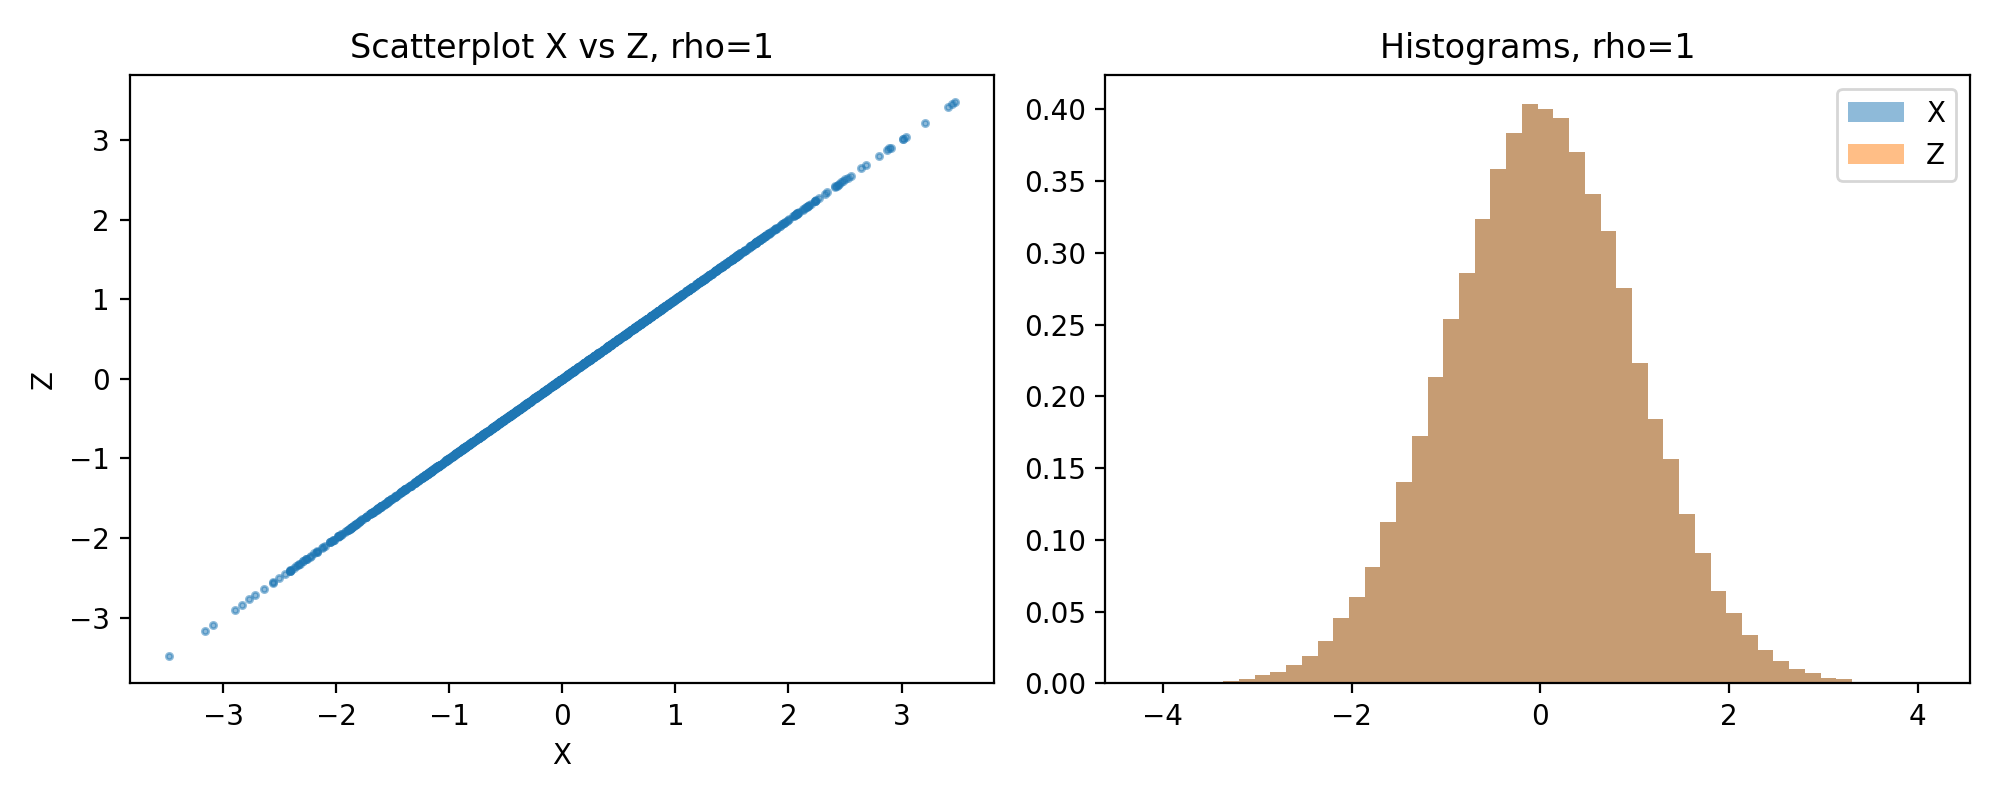
\includegraphics[width=0.9\textwidth]
      {output/gauss_coupling_rho_1.png}
  \end{center}

  \begin{center}
    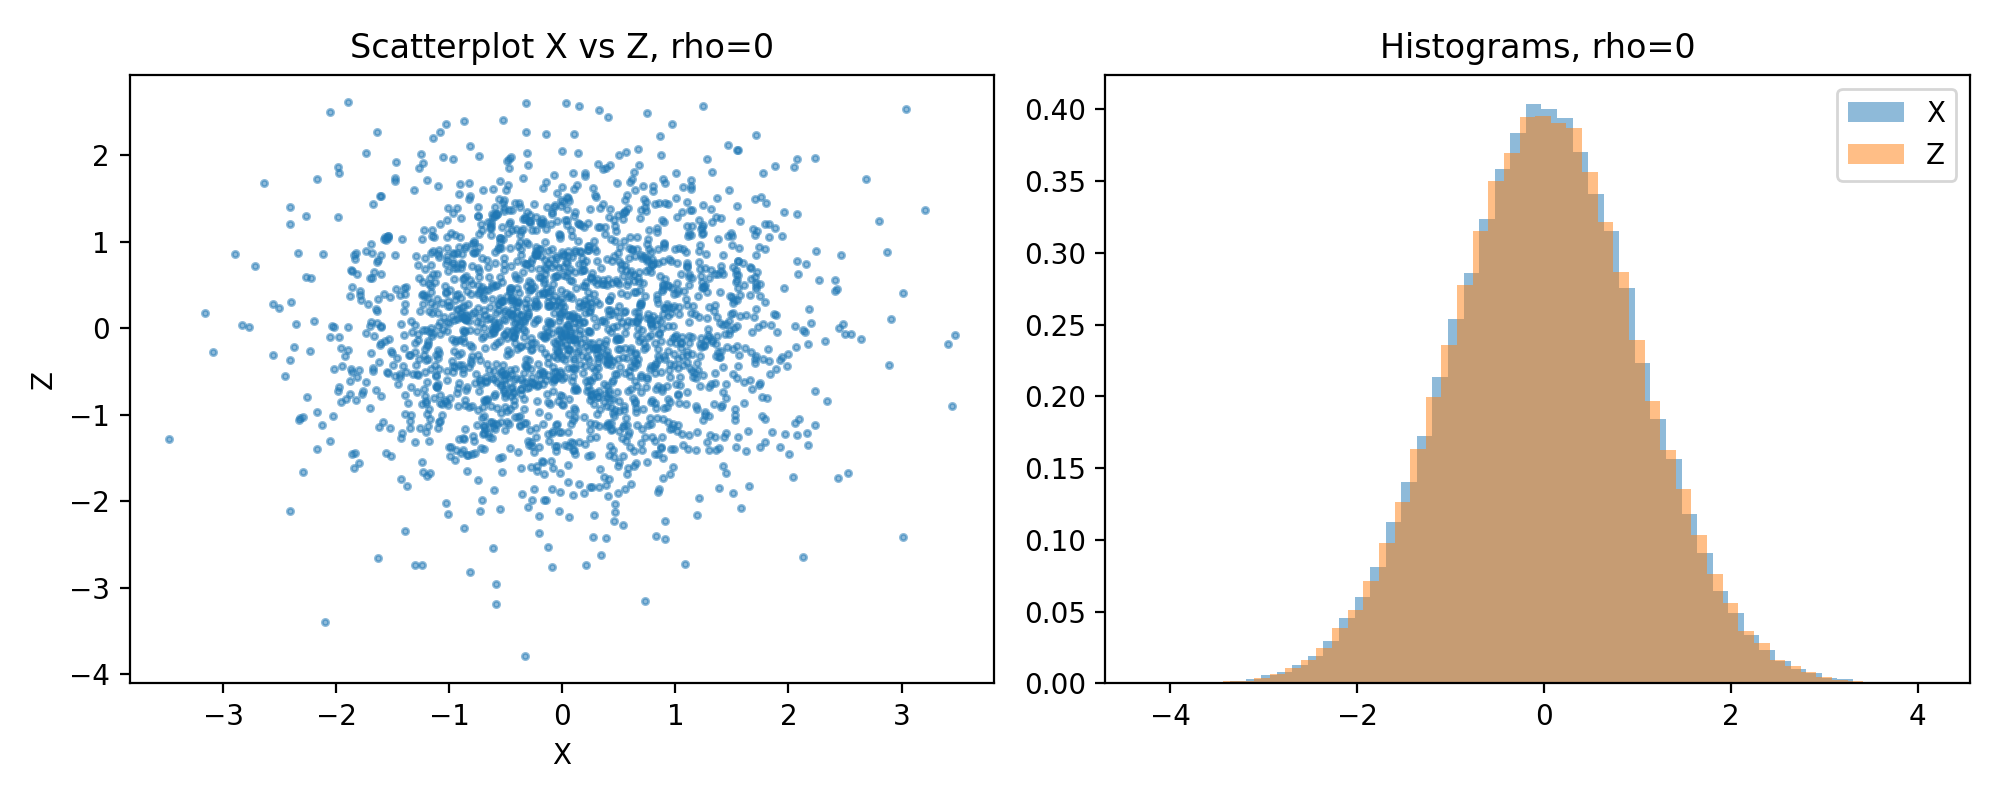
\includegraphics[width=0.9\textwidth]
      {output/gauss_coupling_rho_0.png}
  \end{center}


  \begin{center}
    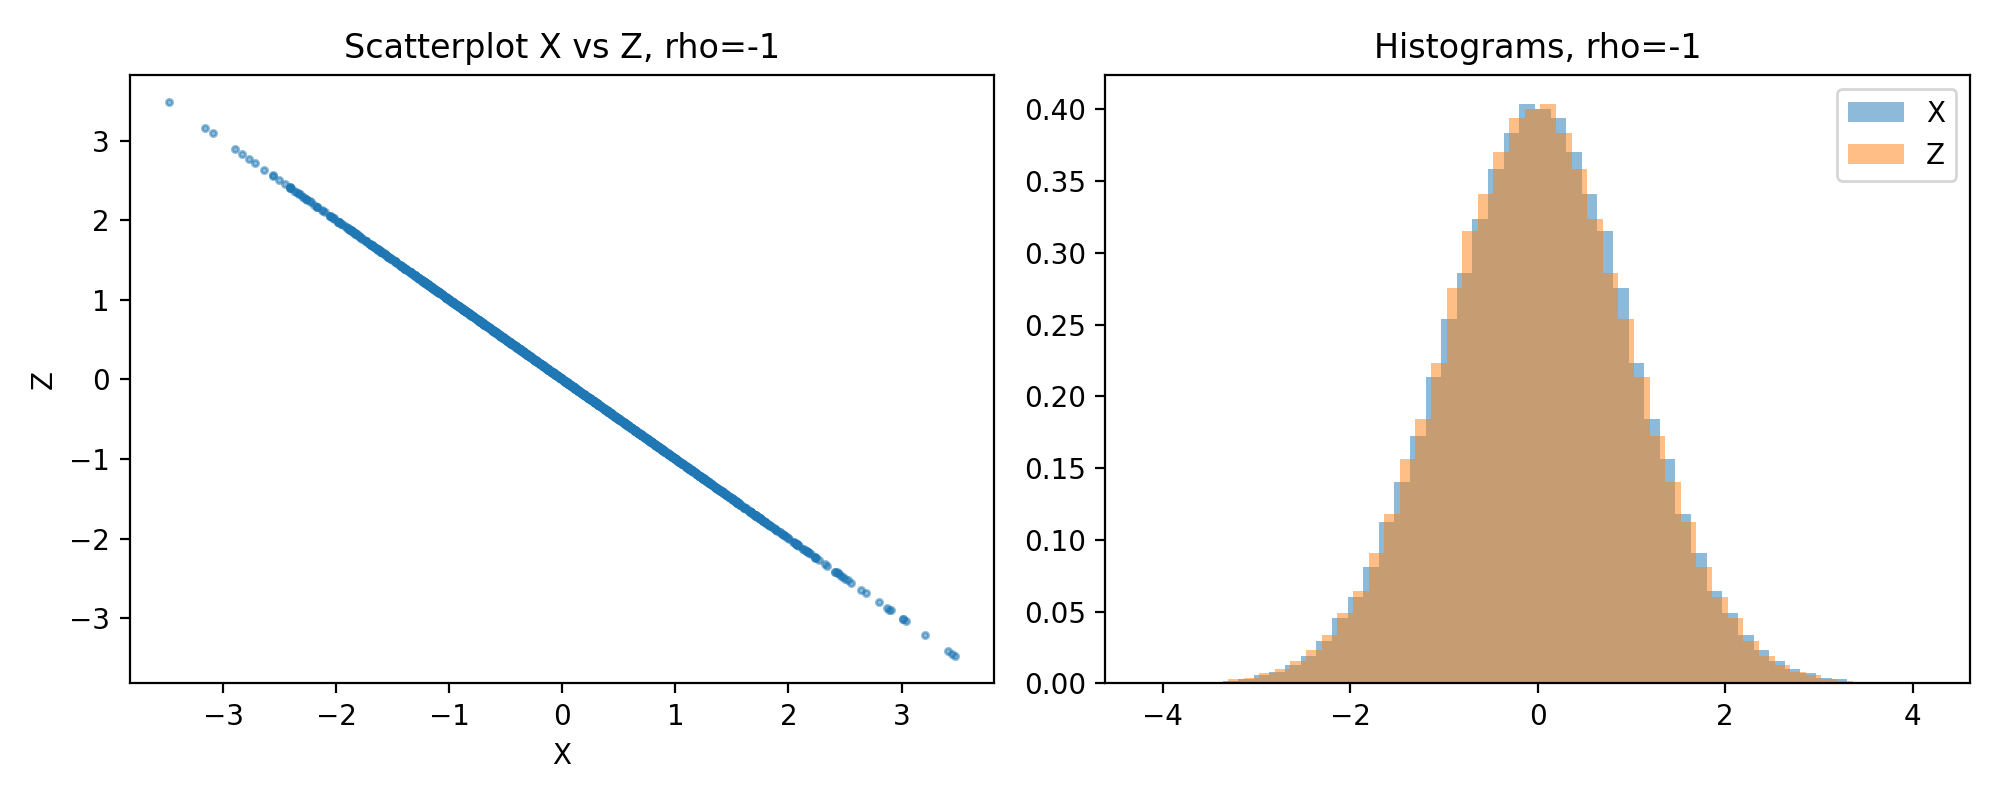
\includegraphics[width=0.9\textwidth]
      {output/gauss_coupling_rho_-1.png}
  \end{center}

In each case, the histograms of $X$ and $Z_\rho$ are nearly
indistinguishable and closely match the standard normal density,
confirming that both marginals are approximately $N(0,1)$.  The
scatterplots show sample correlation close to $\rho$, illustrating how
this coupling interpolates between identical, independent, and
antithetic Gaussian pairs. \qedhere
\end{solution}
  
  \item Consider $(X_1, X_2) = (aX + bY,\,cX + dY)$. Find values of $(a,b,c,d)$ such that:
  \begin{enumerate}
    \item $(X_1, X_2)$ is a coupling of two standard Gaussian random variables;
    \item $X_1 + X_2 = X$.
  \end{enumerate}
  \emph{Remark:} We may interpret $X$ as a fixed Gaussian ``budget'' to be split between $X_1$ and $X_2$, while requiring both parts to still be standard Gaussian.

  \begin{solution}
  Let
  \[
  X_1 = aX + bY, \qquad X_2 = cX + dY.
  \]
  Since $X$ and $Y$ are independent standard normals, requiring $X_1$ and $X_2$ to be standard Gaussian gives
  \[
  a^2 + b^2 = 1, \qquad c^2 + d^2 = 1.
  \]
  The condition $X_1 + X_2 = X$ implies
  \[
  (a+c)X + (b+d)Y = X,
  \]
  so
  \[
  a+c = 1, \qquad b+d = 0.
  \]

  One convenient family of solutions is obtained as follows: choose any $b \in [-1,1]$, set
  \[
  a = \sqrt{1-b^2}, \qquad c = 1-a, \qquad d = -b.
  \]
  Then
  \[
  a^2+b^2=1,
  \]
  and also
  \[
  a+c = a+(1-a)=1, \qquad b+d=b-b=0.
  \]
  Finally,
  \[
  c^2+d^2 = (1-a)^2 + b^2 = 1 - 2a + a^2 + b^2 = 1,
  \]
  because $a^2+b^2=1$. Hence this choice gives a valid coupling of two standard Gaussian random variables satisfying $X_1+X_2=X$.
  \end{solution}
\end{enumerate}

%%%%%%%%%%%%%%%%%%%%%%%%%%%%%%%%%%%%%%%%%%%%%%%%%%%%%%
\section*{Problem 2: Random walk on the complete graph}

Consider the Markov chain on $\Omega = \{1,2,\dots,n\}$ defined as follows: if the chain is currently at state $x$, then it moves uniformly to one of the other $n-1$ states. In other words,
\[
P(x,z) = \frac{1}{n-1}\,\mathbf{1}\{z \neq x\}.
\]

\begin{enumerate}
  \item Show that the uniform distribution on $\Omega$ is stationary for this Markov chain.

  \begin{solution}
  Let $\pi$ be the uniform distribution on $\Omega$, so $\pi(x)=1/n$ for each $x$. For any $z \in \Omega$,
  \[
  (\pi P)(z) = \sum_{x\in\Omega} \pi(x)P(x,z)
  = \sum_{x\neq z} \frac{1}{n}\cdot \frac{1}{n-1}
  = \frac{n-1}{n}\cdot \frac{1}{n-1}
  = \frac{1}{n}
  = \pi(z).
  \]
  Therefore the uniform distribution is stationary.
  \end{solution}

  \item Let $x \neq y$. Compute $\|P(x,\cdot) - P(y,\cdot)\|_{\TV}$.

  \begin{solution}
  By definition,
  \[
  \|P(x,\cdot)-P(y,\cdot)\|_{\TV}
  = \frac12 \sum_{z\in\Omega} |P(x,z)-P(y,z)|.
  \]
  The two distributions differ only at $z=x$ and $z=y$. Indeed,
  \[
  |P(x,x)-P(y,x)| = \left|0-\frac{1}{n-1}\right| = \frac{1}{n-1},
  \]
  and
  \[
  |P(x,y)-P(y,y)| = \left|\frac{1}{n-1}-0\right| = \frac{1}{n-1}.
  \]
  Thus
  \[
  \|P(x,\cdot)-P(y,\cdot)\|_{\TV}
  = \frac12\left(\frac{1}{n-1}+\frac{1}{n-1}\right)
  = \frac{1}{n-1}.
  \]
  \end{solution}

  \item Construct a coupling $(X_1,Y_1)$ of $P(x,\cdot)$ and $P(y,\cdot)$ such that
  \[
  \mathbb{P}(X_1 \neq Y_1) = \|P(x,\cdot) - P(y,\cdot)\|_{\TV}.
  \]

\begin{solution}
Define a coupling of $P(x,\cdot)$ and $P(y,\cdot)$ as follows.

\begin{itemize}
  \item With probability $\frac{1}{n-1}$, set $(X_1,Y_1) = (y,x)$.
  \item With the remaining probability $1 - \frac{1}{n-1}$, choose
        $Z$ uniformly from $\Omega \setminus \{x,y\}$ and set
        $(X_1,Y_1) = (Z,Z)$.
\end{itemize}

We first check that the marginals are correct.

For the $X$-marginal:
\[
  \mathbb{P}(X_1 = y)
  = \frac{1}{n-1}, \qquad
  \mathbb{P}(X_1 = x)
  = 0,
\]
and for any $z \in \Omega \setminus \{x,y\}$,
\[
  \mathbb{P}(X_1 = z)
  = \left(1 - \frac{1}{n-1}\right)
    \mathbb{P}(Z = z)
  = \frac{n-2}{n-1} \cdot \frac{1}{n-2}
  = \frac{1}{n-1}.
\]
Thus $X_1$ is uniform on $\Omega \setminus \{x\}$, so
$X_1 \sim P(x,\cdot)$.  A symmetric argument shows
$Y_1 \sim P(y,\cdot)$.

Next, we compute the disagreement probability under this coupling.
Disagreement occurs only in the first case, when $(X_1,Y_1) = (y,x)$.
Hence
\[
  \mathbb{P}(X_1 \neq Y_1)
  = \frac{1}{n-1}.
\]
From part (2), we already know that
$\|P(x,\cdot) - P(y,\cdot)\|_{\mathrm{TV}} = \frac{1}{n-1}$, so this
coupling satisfies
\[
  \mathbb{P}(X_1 \neq Y_1)
  = \|P(x,\cdot) - P(y,\cdot)\|_{\mathrm{TV}},
\]
as required. 
\end{solution}

  \item Now run this coupling at every step. Let
  \[
  T := \inf\{t \ge 0 : X_t = Y_t\}.
  \]
  Show that if $X_0 \neq Y_0$, then
  \[
  \mathbb{P}(T > t) = \left(\frac{1}{n-1}\right)^t.
  \]

\begin{solution}
We run at every step the coupling from part (3), and define
\[
  T := \inf\{t \ge 0 : X_t = Y_t\}.
\]
We show that for $x \neq y$,
\[
  \mathbb{P}(T > t) = \left(\frac{1}{n-1}\right)^{t}.
\]

From the construction in part (3), whenever $X_t \neq Y_t$, the one–step
coupling satisfies
\[
  \mathbb{P}(X_{t+1} \neq Y_{t+1} \mid X_t \neq Y_t)
  = \frac{1}{n-1}.
\]
Moreover, once the chains meet, the coupling keeps them together
forever: if $X_t = Y_t$ then $X_{t'} = Y_{t'}$ for all $t' \ge t$.

We now prove the formula by induction on $t$.

\medskip\noindent
\textit{Base case.} For $t=0$ and $x \neq y$ we have $T > 0$
almost surely, so $\mathbb{P}(T>0) = 1 = (1/(n-1))^{0}$.

\medskip\noindent
\textit{Inductive step.} Assume
$\mathbb{P}(T > t) = (1/(n-1))^{t}$ for some $t \ge 0$. Then
\[
  \mathbb{P}(T > t+1)
  = \mathbb{P}(T > t+1 \mid T > t)\,\mathbb{P}(T > t)
  = \mathbb{P}(X_{t+1} \neq Y_{t+1} \mid X_t \neq Y_t)\,
    \mathbb{P}(T > t),
\]
where we used that $T > t$ is equivalent to $X_t \neq Y_t$ and the
Markov property of the coupled chain. By the one–step calculation above,
\[
  \mathbb{P}(X_{t+1} \neq Y_{t+1} \mid X_t \neq Y_t)
  = \frac{1}{n-1},
\]
so
\[
  \mathbb{P}(T > t+1)
  = \frac{1}{n-1} \cdot \left(\frac{1}{n-1}\right)^{t}
  = \left(\frac{1}{n-1}\right)^{t+1}.
\]
This completes the induction and proves the claim. \qedhere
\end{solution}

  \item Use the coupling inequality to conclude that
  \[
  \max_{x,y} \|P^t(x,\cdot) - P^t(y,\cdot)\|_{\TV}
  \le \left(\frac{1}{n-1}\right)^t.
  \]

  \begin{solution}
  By the coupling inequality,
  \[
  \|P^t(x,\cdot)-P^t(y,\cdot)\|_{\TV} \le \mathbb{P}(T>t).
  \]
  Using the coupling from the previous parts,
  \[
  \mathbb{P}(T>t)=\left(\frac{1}{n-1}\right)^t.
  \]
  Hence
  \[
  \max_{x,y} \|P^t(x,\cdot)-P^t(y,\cdot)\|_{\TV}
  \le \left(\frac{1}{n-1}\right)^t.
  \]
  \end{solution}
\end{enumerate}

%%%%%%%%%%%%%%%%%%%%%%%%%%%%%%%%%%%%%%%%%%%%%%%%%%%%%%
\section*{Problem 3: Random-to-top shuffle}

Consider a deck of $n$ cards labeled $1,\dots,n$. A shuffling is a permutation of $\{1,2,\dots,n\}$. For example, if $n=5$, then $(5,1,4,3,2)$ means the fifth card is on the top of the deck, followed by the first card, and so on. We say a shuffle mixes the deck if, after a number of steps, the distribution of the permutation is close to the uniform distribution over all $n!$ permutations.

The random-to-top shuffle is the following Markov chain on permutations: at each step, choose one card label uniformly at random from $\{1,\dots,n\}$, remove that card from its current position, and move it to the top of the deck.

\begin{enumerate}
  \item Show that the uniform distribution on all $n!$ permutations is stationary for this Markov chain.

 \begin{solution}
  Let $\pi$ be the uniform distribution on $S_n$, so 
$\pi(\sigma) = \frac{1}{n!}$ for each $\sigma \in S_n$. We verify the 
balance equation $\pi P = \pi$ directly.

Fix any $\tau \in S_n$. We compute
\[
    (\pi P)(\tau) = \sum_{\sigma \in S_n} \pi(\sigma)\, P(\sigma, \tau).
\]
We need to identify the permutations $\sigma$ for which $P(\sigma, \tau) > 0$,
i.e., those from which a single random-to-top move can produce $\tau$.
Such a $\sigma$ is obtained by taking $\tau$ and inserting its top card back
into one of the $n$ positions in the deck. There are exactly $n$ such
permutations $\sigma_1, \ldots, \sigma_n$, and for each one the transition
probability is $P(\sigma_k, \tau) = \frac{1}{n}$ (the card on top of $\tau$
is chosen with probability $\frac{1}{n}$).

Therefore,
\[
    (\pi P)(\tau)
    = \sum_{k=1}^{n} \pi(\sigma_k)\cdot P(\sigma_k,\tau)
    = \sum_{k=1}^{n} \frac{1}{n!} \cdot \frac{1}{n}
    = \frac{n}{n \cdot n!}
    = \frac{1}{n!}
    = \pi(\tau).
\]
Hence $\pi P = \pi$, so the uniform distribution is stationary. 
 \end{solution} 

  \item Let $X_t$ and $Y_t$ be two copies of the random-to-top shuffle, started from two possibly different initial decks $X_0$ and $Y_0$. Couple them by choosing the same card label at every step and moving that label to the top in both decks.

  Let $A_t$ be the set of card labels that have been chosen at least once by time $t$. Show that the relative order of the cards in $A_t$ is the same in $X_t$ and $Y_t$.

  \begin{solution}
We prove the claim by induction on $t$. For $t = 0$, the set $A_0$ is
empty, so the statement is trivial.

Assume the claim holds at time $t$, and consider time $t+1$. Let $i_{t+1}$
be the label chosen at step $t+1$.

\medskip\noindent
\textit{Case 1: $i_{t+1} \in A_t$.}
Then in both decks we move the same card $i_{t+1}$ to the top. In each
deck, the positions of all other labels in $A_t$ do not change; only
$i_{t+1}$ moves above them. Since the relative order of the labels in
$A_t$ was the same in $X_t$ and $Y_t$ by the induction hypothesis, and
we apply the same operation to $i_{t+1}$ in both decks, the relative
order of the labels in $A_t$ remains the same in $X_{t+1}$ and $Y_{t+1}$.
In this case $A_{t+1} = A_t$.

\medskip\noindent
\textit{Case 2: $i_{t+1} \notin A_t$.}
Then $A_{t+1} = A_t \cup \{i_{t+1}\}$, and in both decks the new label
$i_{t+1}$ is moved to the top of the deck. In particular, $i_{t+1}$ is
placed above all labels in $A_t$ in both $X_{t+1}$ and $Y_{t+1}$, while
the relative order of the labels in $A_t$ among themselves is unchanged.
Thus the relative order of the labels in $A_{t+1}$ is the same in
$X_{t+1}$ and $Y_{t+1}$.

\medskip

In either case, the relative order of the labels in $A_{t+1}$ is the
same in the two decks. By induction, the claim holds for all $t$. \qedhere
\end{solution}

  \item Show that if $A_t = \{1,\dots,n\}$, then $X_t = Y_t$. Let
  \[
  T := \inf\{t \ge 0 : X_t = Y_t\}.
  \]
  Deduce that
  \[
  \mathbb{P}(T > t) \le \mathbb{P}(A_t \neq \{1,\dots,n\}).
  \]

  \begin{solution}
  If $A_t=\{1,\dots,n\}$, then every label has been selected at least once. By the previous part, the relative order of all labels is then the same in $X_t$ and $Y_t$, so $X_t=Y_t$.

  Therefore, if $T>t$, then necessarily $A_t\neq \{1,\dots,n\}$. Hence
  \[
  \mathbb{P}(T>t) \le \mathbb{P}(A_t\neq \{1,\dots,n\}).
  \]
  \end{solution}

  \item Use the union bound to prove that
  \[
  \mathbb{P}(A_t \neq \{1,\dots,n\})
  \le n\left(1 - \frac{1}{n}\right)^t
  \le ne^{-t/n}.
  \]

  \begin{solution}
  For each label $i$, let $E_i$ be the event that label $i$ has not been chosen by time $t$. Then
  \[
  \mathbb{P}(E_i)=\left(1-\frac{1}{n}\right)^t.
  \]
  If $A_t\neq\{1,\dots,n\}$, then at least one $E_i$ occurs. By the union bound,
  \[
  \mathbb{P}(A_t\neq\{1,\dots,n\}) \le \sum_{i=1}^n \mathbb{P}(E_i)
  = n\left(1-\frac{1}{n}\right)^t.
  \]
  Using $1-1/n \le e^{-1/n}$ gives
  \[
  \mathbb{P}(A_t\neq\{1,\dots,n\}) \le ne^{-t/n}.
  \]
  \end{solution}

  \item Using the coupling inequality, conclude that
  \[
  \max_{x,y} \|P^t(x,\cdot) - P^t(y,\cdot)\|_{\TV}
  \le ne^{-t/n}.
  \]
  In particular, show that the mixing time is at most
  \[
  t_{\mathrm{mix}}(\varepsilon) \le n \log n + n \log(1/\varepsilon).
  \]

  \begin{solution}
  By the coupling inequality and the previous bounds,
  \[
  \max_{x,y}\|P^t(x,\cdot)-P^t(y,\cdot)\|_{\TV}
  \le \mathbb{P}(T>t)
  \le \mathbb{P}(A_t\neq\{1,\dots,n\})
  \le ne^{-t/n}.
  \]
  To make this at most $\varepsilon$, it suffices that
  \[
  ne^{-t/n} \le \varepsilon.
  \]
  Taking logarithms yields
  \[
  t \ge n\log n + n\log(1/\varepsilon).
  \]
  Therefore,
  \[
  t_{\mathrm{mix}}(\varepsilon) \le n\log n + n\log(1/\varepsilon).
  \]
  \end{solution}
\end{enumerate}

%%%%%%%%%%%%%%%%%%%%%%%%%%%%%%%%%%%%%%%%%%%%%%%%%%%%%%
\section*{Problem 4: Conditional Bernoulli distribution}

In this problem, we study an MCMC algorithm for sampling from the conditional Bernoulli distribution. Fix two positive integers $0 < I < N$ and parameters $(p_1,\dots,p_N) \in (0,1)^N$. The conditional Bernoulli distribution is the distribution on binary vectors $\{0,1\}^N$ defined by
\[
\mathbb{P}(X_1=x_1,\dots,X_N=x_N)
\propto \prod_{k=1}^N p_k^{x_k}(1-p_k)^{1-x_k}\,\mathbf{1}\!\left(\sum_{i=1}^N x_i=I\right).
\]
Equivalently, it is the distribution of independent Bernoulli random variables $X_k \sim \operatorname{Ber}(p_k)$ conditioned on $\sum_{i=1}^N X_i = I$.

We now consider the following MCMC algorithm. Given a current state $x^{(t)} \in \{0,1\}^N$ satisfying $\sum_{i=1}^N x_i^{(t)} = I$, define
\[
S_0(t):=\{i:x_i^{(t)}=0\}, \qquad S_1(t):=\{j:x_j^{(t)}=1\}.
\]
At each iteration, choose $i_t \in S_0(t)$ and $j_t \in S_1(t)$ independently and uniformly at random. The proposal flips the two coordinates $x^{(t)}_{i_t}$ and $x^{(t)}_{j_t}$, and is then accepted or rejected according to the Metropolis--Hastings rule.

\begin{enumerate}
  \item Calculate the acceptance probability for a proposed flip of coordinates $i_t$ and $j_t$.

\begin{solution}
Let $x \in \mathcal{X}$ be the current state and let $y$ be obtained by
changing $x_i = 0$ to $y_i = 1$ and $x_j = 1$ to $y_j = 0$, for some
$i \in S_0(x)$ and $j \in S_1(x)$. Since $|S_0(x)| = N-I$ and
$|S_1(x)| = I$, the proposal probability is
\[
  q(x,y) = \frac{1}{|S_0(x)|}\,\frac{1}{|S_1(x)|}
         = \frac{1}{(N-I)\,I}.
\]
The reverse move $y \to x$ has the same proposal probability, so
$q(y,x) = q(x,y)$. Therefore the Metropolis–Hastings acceptance
probability is
\[
  \alpha(x,y) = \min\Bigl\{1,\, \frac{\pi(y)}{\pi(x)}\Bigr\}.
\]

Since $\pi$ is proportional to
$ \prod_{k=1}^N p_k^{x_k} (1-p_k)^{1-x_k} $
restricted to $\sum_{k=1}^N x_k = I$, the normalizing constant cancels in
the ratio, and only coordinates $i$ and $j$ differ between $x$ and $y$.
Thus
\[
  \frac{\pi(y)}{\pi(x)}
  = \frac{p_i^{y_i}(1-p_i)^{1-y_i}\,p_j^{y_j}(1-p_j)^{1-y_j}}
         {p_i^{x_i}(1-p_i)^{1-x_i}\,p_j^{x_j}(1-p_j)^{1-x_j}}
  = \frac{p_i}{1-p_i} \cdot \frac{1-p_j}{p_j}.
\]
Hence
\[
  \alpha(x,y)
  = \min\left\{1,\,
      \frac{p_i}{1-p_i}\cdot\frac{1-p_j}{p_j}
    \right\}. 
  \]
\end{solution}

  \item Prove that the Markov chain is irreducible on
  \[
  \mathcal{X} := \left\{x \in \{0,1\}^N : \sum_{i=1}^N x_i = I\right\}.
  \]

  \begin{solution}
Take any $x,y \in \mathcal{X}$. Let
\[
  A = \{k : x_k = 1,\ y_k = 0\},
  \qquad
  B = \{k : x_k = 0,\ y_k = 1\}.
\]
Since both $x$ and $y$ have exactly $I$ ones, we have $|A| = |B|$. Pair
the elements of $A$ and $B$ arbitrarily, say $(a_1,b_1),\dots,(a_m,b_m)$
with $m = |A|$.

Starting from $x$, for $\ell = 1,\dots,m$ perform the following move:
set the coordinate at $a_\ell$ from $1$ to $0$ and the coordinate at
$b_\ell$ from $0$ to $1$. Each such move is exactly of the allowed form
in the Markov chain (flipping one $0$ to $1$ and one $1$ to $0$), so
every intermediate state lies in $\mathcal{X}$ and has exactly $I$ ones.

After performing all $m$ moves, we obtain $y$, because all coordinates
where $x$ and $y$ differ have been corrected. Each of these moves has
strictly positive proposal probability and strictly positive acceptance
probability since every $p_k \in (0,1)$. Hence there is a positive–probability
path from $x$ to $y$, so the chain is irreducible on $\mathcal{X}$. \qedhere
\end{solution}

  \item Assume there exist constants $0 < c < C < \infty$ such that
  \[
  c < \frac{p_k}{1-p_k} < C
  \qquad\text{for every } k = 1,\dots,N.
  \]
  Prove that the above algorithm has mixing time
  \[
  t_{\mathrm{mix}}(\varepsilon) = O(N \log N).
  \]

  \begin{solution}
We use path coupling. Define a graph on $\mathcal{X}$ where $x \sim y$ if
they differ in exactly two coordinates (one $0 \to 1$ and one $1 \to 0$),
and let
\[
  \ell(x,y) = \frac{1}{2}\sum_{k=1}^N |x_k - y_k|
\]
be the (Hamming) distance. It suffices to consider neighboring states
$x,y$ with $\ell(x,y) = 1$, i.e., there exist unique indices $u,v$ such
that
\[
  x_u = 1,\quad x_v = 0, \qquad y_u = 0,\quad y_v = 1,
\]
and $x_k = y_k$ for all $k \neq u,v$.

\medskip\noindent
\textit{Coupled proposal.}
At each step, draw the same pair $(i_t,j_t)$, with $i_t \in S_0(x)$,
$j_t \in S_1(x)$ for the $x$–chain, and couple the $y$–chain so that it
uses the same pair whenever valid (i.e.\ when $i_t \in S_0(y)$ and
$j_t \in S_1(y)$ as well). Since $x$ and $y$ differ only at $u,v$, we
have
\[
  S_0(x) \triangle S_0(y) = \{u,v\},
  \qquad
  S_1(x) \triangle S_1(y) = \{u,v\}.
\]

\medskip\noindent
\textit{Drift computation.}
There are three types of proposed moves:

\begin{itemize}
\item \emph{Coalescing move} $(i_t,j_t) = (v,u)$: this is the unique
  proposal that swaps the disagreement and makes the two chains
  coincide. It is chosen with probability
  \[
    \frac{1}{|S_0(x)|\,|S_1(x)|} = \frac{1}{(N-I)\,I}.
  \]
  The Metropolis–Hastings acceptance probability for this move in the
  $x$–chain is
  \[
    \alpha(x,x') = \min\!\left\{1,\,
      \frac{p_v}{1-p_v}\cdot\frac{1-p_u}{p_u}
    \right\}.
  \]
  By the assumption $c < p_k/(1-p_k) < C$ for all $k$, the ratio inside
  the minimum lies in $(c/C,\, C/c)$, so there exists
  $\alpha_0 := \min(1,c/C) > 0$ such that $\alpha(x,x') \ge \alpha_0$.
  If both chains accept this move, $\ell$ decreases by $1$. Thus this
  case contributes at most
  \[
    -\frac{\alpha_0}{(N-I)\,I}
  \]
  to the expected change in $\ell$.

\item \emph{Neutral moves} (neither $i_t$ nor $j_t$ is in $\{u,v\}$):
  the same coordinates are proposed and updated in both chains, and the
  accept/reject decisions are the same under our coupling. Hence
  $\ell(X_1,Y_1) = \ell(X_0,Y_0)$, and these moves contribute $0$ to the
  drift.

\item \emph{Discordant moves} (exactly one of $i_t,j_t$ lies in
  $\{u,v\}$): in this case the two chains may update different
  coordinates. There are $O(N)$ such pairs $(i_t,j_t)$, each chosen with
  probability at most $1/((N-I)\,I)$, and in the worst case $\ell$ can
  increase by at most $1$. Thus the total positive contribution to the
  drift from discordant moves is bounded above by
  \[
    \frac{C_1}{(N-I)\,I}
  \]
  for some constant $C_1$ independent of $N$.
\end{itemize}

Putting these together, for neighboring $x,y$ we obtain
\[
  \mathbb{E}\!\left[\ell(X_1,Y_1) - \ell(X_0,Y_0)
    \,\middle|\, X_0 = x,\, Y_0 = y\right]
  \le -\frac{\alpha_0 - C_1}{(N-I)\,I}.
\]
Since $I(N-I) \asymp N$ and $\alpha_0$ depends only on $c,C$, by
absorbing constants we can choose $\kappa > 0$ (depending only on
$c,C$) such that, for all sufficiently large $N$,
\[
  \mathbb{E}[\ell(X_1,Y_1) \mid X_0=x,Y_0=y]
  \le \ell(x,y)\left(1 - \frac{\kappa}{N}\right)
  = 1 - \frac{\kappa}{N}.
\]

\medskip\noindent
\textit{Conclusion.}
By the path coupling theorem, for any $x,y \in \mathcal{X}$ and any
$t \ge 0$,
\[
  \mathbb{E}[\ell(X_t,Y_t)]
  \le \ell(x,y)\left(1 - \frac{\kappa}{N}\right)^t
  \le N\left(1 - \frac{\kappa}{N}\right)^t
  \le N e^{-\kappa t/N}.
\]
Since
\[
  \|P^t(x,\cdot) - P^t(y,\cdot)\|_{\mathrm{TV}}
  \le \mathbb{P}(X_t \neq Y_t)
  \le \mathbb{E}[\ell(X_t,Y_t)],
\]
we obtain
\[
  \max_{x,y} \|P^t(x,\cdot) - P^t(y,\cdot)\|_{\mathrm{TV}}
  \le N e^{-\kappa t/N}.
\]
Solving $N e^{-\kappa t/N} \le \varepsilon$ for $t$ gives
\[
  t \;\ge\; \frac{N}{\kappa}\bigl(\log N + \log(1/\varepsilon)\bigr),
\]
so the mixing time satisfies
\[
  t_{\mathrm{mix}}(\varepsilon) = O(N \log N). \qedhere
\]
\end{solution}
\end{enumerate}

\end{document}